\ifx\allfiles\undefined
\documentclass[12pt, a4paper,oneside, UTF8]{ctexbook}
\usepackage[dvipsnames]{xcolor}
\usepackage{mathtools}   % 数学公式(mathtools 是 amsmath 的上位替代)
\usepackage{amsthm}    % 定理环境
\usepackage{amssymb}   % 更多公式符号
\usepackage{graphicx}  % 插图
%\usepackage{mathrsfs}  % 数学字体
%\usepackage{newtxtext,newtxmath}
%\usepackage{arev}
\usepackage{kmath,kerkis}
\usepackage{newtxtext}
\usepackage{bbm}
\usepackage{enumitem}  % 列表
\usepackage{geometry}  % 页面调整
%\usepackage{unicode-math}
\usepackage[colorlinks,linkcolor=black]{hyperref}

\usepackage{wrapfig}


\usepackage{ulem}	   % 用于更多的下划线格式,
					   % \uline{}下划线,\uuline{}双下划线,\uwave{}下划波浪线,\sout{}中间删除线,\xout{}斜删除线
					   % \dashuline{}下划虚线,\dotuline{}文字底部加点


\graphicspath{ {flg/},{../flg/}, {config/}, {../config/} }  % 配置图形文件检索目录
\linespread{1.5} % 行高

% 页码设置
\geometry{top=25.4mm,bottom=25.4mm,left=20mm,right=20mm,headheight=2.17cm,headsep=4mm,footskip=12mm}

% 设置列表环境的上下间距
\setenumerate[1]{itemsep=5pt,partopsep=0pt,parsep=\parskip,topsep=5pt}
\setitemize[1]{itemsep=5pt,partopsep=0pt,parsep=\parskip,topsep=5pt}
\setdescription{itemsep=5pt,partopsep=0pt,parsep=\parskip,topsep=5pt}

% 定理环境
% ########## 定理环境 start ####################################
\theoremstyle{definition}
\newtheorem{defn}{\indent 定义}[section]

\newtheorem{lemma}{\indent 引理}[section]    % 引理 定理 推论 准则 共用一个编号计数
\newtheorem{thm}[lemma]{\indent 定理}
\newtheorem{corollary}[lemma]{\indent 推论}
\newtheorem{criterion}[lemma]{\indent 准则}

\newtheorem{proposition}{\indent 命题}[section]
\newtheorem{example}{\indent \color{SeaGreen}{例}}[section] % 绿色文字的 例 ,不需要就去除\color{SeaGreen}{}
\newtheorem*{rmk}{\indent \color{red}{注}}

% 两种方式定义中文的 证明 和 解 的环境:
% 缺点:\qedhere 命令将会失效【技术有限,暂时无法解决】
\renewenvironment{proof}{\par\textbf{证明.}\;}{\qed\par}
\newenvironment{solution}{\par{\textbf{解.}}\;}{\qed\par}

% 缺点:\bf 是过时命令,可以用 textb f等替代,但编译会有关于字体的警告,不过不影响使用【技术有限,暂时无法解决】
%\renewcommand{\proofname}{\indent\bf 证明}
%\newenvironment{solution}{\begin{proof}[\indent\bf 解]}{\end{proof}}
% ######### 定理环境 end  #####################################

% ↓↓↓↓↓↓↓↓↓↓↓↓↓↓↓↓↓ 以下是自定义的命令  ↓↓↓↓↓↓↓↓↓↓↓↓↓↓↓↓

% 用于调整表格的高度  使用 \hline\xrowht{25pt}
\newcommand{\xrowht}[2][0]{\addstackgap[.5\dimexpr#2\relax]{\vphantom{#1}}}

% 表格环境内长内容换行
\newcommand{\tabincell}[2]{\begin{tabular}{@{}#1@{}}#2\end{tabular}}

% 使用\linespread{1.5} 之后 cases 环境的行高也会改变,重新定义一个 ca 环境可以自动控制 cases 环境行高
\newenvironment{ca}[1][1]{\linespread{#1} \selectfont \begin{cases}}{\end{cases}}
% 和上面一样
\newenvironment{vx}[1][1]{\linespread{#1} \selectfont \begin{vmatrix}}{\end{vmatrix}}

\def\d{\textup{d}} % 直立体 d 用于微分符号 dx
\def\R{\mathbb{R}} % 实数域
\def\N{\mathbb{N}} % 自然数域
\def\C{\mathbb{C}} % 复数域
\def\Z{\mathbb{Z}} % 整数环
\def\Q{\mathbb{Q}} % 有理数域
\newcommand{\bs}[1]{\boldsymbol{#1}}    % 加粗,常用于向量
\newcommand{\ora}[1]{\overrightarrow{#1}} % 向量

% 数学 平行 符号
\newcommand{\pll}{\kern 0.56em/\kern -0.8em /\kern 0.56em}

% 用于空行\myspace{1} 表示空一行 填 2 表示空两行  
\newcommand{\myspace}[1]{\par\vspace{#1\baselineskip}}

%s.t. 用\st就能打出s.t.
\DeclareMathOperator{\st}{s.t.}

%罗马数字 \rmnum{}是小写罗马数字, \Rmnum{}是大写罗马数字
\makeatletter
\newcommand{\rmnum}[1]{\romannumeral #1}
\newcommand{\Rmnum}[1]{\expandafter@slowromancap\romannumeral #1@}
\makeatother
\begin{document}
	% \title{{\Huge{\textbf{$Partial \,\, Differential \,\, Equations$}}}\footnote{参考书籍:\\
			\hspace*{4em} \textbf{《Partial Differential Equations》 -- Lawrence C. Evans} \\
			\hspace*{4em} \textbf{《Partial Differential Equations》 -- Fritz John} \\
			\hspace*{4em} \textbf{《数学物理方程讲义 (第二版)》--  姜礼尚、陈亚浙、刘西垣、易法槐} 
			}}
\author{$-TW-$}
\date{\today}
\maketitle                   % 在单独的标题页上生成一个标题

\thispagestyle{empty}        % 前言页面不使用页码
\begin{center}
	\Huge\textbf{序}
\end{center}


\vspace*{3em}
\begin{center}
	\large{\textbf{天道几何,万品流形先自守;}}\\
	
	\large{\textbf{变分无限,孤心测度有同伦。}}
\end{center}

\vspace*{3em}
\begin{flushright}
	\begin{tabular}{c}
		\today \\ \small{\textbf{长夜伴浪破晓梦,梦晓破浪伴夜长}}
	\end{tabular}
\end{flushright}


\newpage                      % 新的一页
\pagestyle{plain}             % 设置页眉和页脚的排版方式(plain:页眉是空的,页脚只包含一个居中的页码)
\setcounter{page}{1}          % 重新定义页码从第一页开始
\pagenumbering{Roman}         % 使用大写的罗马数字作为页码
\tableofcontents              % 生成目录

\newpage                      % 以下是正文
\pagestyle{plain}
\setcounter{page}{1}          % 使用阿拉伯数字作为页码
\pagenumbering{arabic}
\setcounter{chapter}{0}    % 设置 -1 可作为第零章绪论从第零章开始 
	\else
	\fi
	%  ############################ 正文部分
\appendix
\chapter{$Supplementary \,\, Content$}\label{appendix A}

\section{区域边界的光滑性}
	下面我们来给出\textbf{区域边界的光滑性}的定义.
	
	\begin{defn}\label{def A.1.1}
		Suppose $\Omega \subset \R^n$ is open, $\partial \Omega \neq \varnothing$. 如果对于$\forall p \in \partial \Omega$, $\exists p$ 的邻域$U$, $\st$ 在适当的空间直角坐标系下, 
		\begin{align}
			\partial \Omega \cap U &= \{ (x^{'} , x^{n}) \in \R^{n - 1} \times \R \mid x^{'} \in D , \,\, x^n = \varphi(x^{'}) \} \\
			\Omega \cap U &= \{ (x^{'} , x^n) \in \R^{n - 1} \times \R \mid x^{'} \in D , \,\, x^n > \varphi(x^{'}) \} \cap U
		\end{align}
		where $\varphi \in C^{k}(\Omega) , \,\, D \subset \R^{n - 1}$ open. 我们称\underline{\textcolor{blue}{\textbf{$\partial \Omega \in C^k$}}}, 这里$k = 0 , 1 , 2 , \cdots$ 或$\infty$.
		
		\begin{figure}[thbp!]
			\centering
			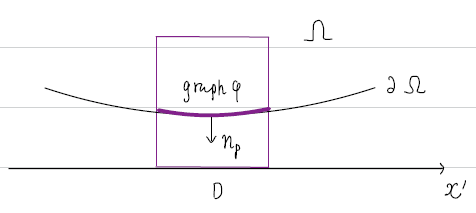
\includegraphics[width=0.5\linewidth]{figure/A.1-1}
			\caption{边界的光滑性}
			\label{pic : A.1-1} % 添加图像引用标签
		\end{figure}
		
		\begin{rmk}
			在\textbf{定义 \ref{def A.1.1}} 中, 设$k \leq 1$, $\,\, x_{0}^{'} \in \partial \Omega$, $\,\, p = (x_{0}^{'} , \varphi(x_{0}^{'}))$. 记
			\[ n_p = \frac{(\nabla \varphi(x_{0}^{'}) , -1)}{\sqrt{1 + \left| \nabla \varphi(x_{0}^{'}) \right|^2}} \]
			称$n_p$ 为$\partial \Omega$ 在$p$ 点的\underline{\textcolor{blue}{\textbf{单位外法向}}}. $n_p$ 的定义与空间直角坐标系的选择无关. 记
			\begin{align}
				n : \partial \Omega &\longrightarrow \R^n \\
				p &\longmapsto n(p) = n_p 
			\end{align}
			称$n$ 为$\partial \Omega$ 的\underline{\textcolor{blue}{\textbf{单位外法向}}}. 因为$\partial \Omega \in C^k$, $k \geq 1$, 所以$n \in C(\partial \Omega ; \R^n)$.
		\end{rmk}
		
		
	\end{defn}







	%  ############################
	\ifx\allfiles\undefined
\end{document}
\fi